%\documentclass[a4paper,twocolumn]{article} % Document type

\documentclass[a4paper,12pt,oneside,onecolumn]{article} % Document type

\usepackage[left=1.0in, right=1.0in, top=1.0in, bottom=1.0in]{geometry}

\ifx\pdfoutput\undefined
    %Use old Latex if PDFLatex does not work
   \usepackage[dvips]{graphicx}% To get graphics working
   \DeclareGraphicsExtensions{.eps} % Encapsulated PostScript
 \else
    %Use PDFLatex
   \usepackage[pdftex]{graphicx}% To get graphics working
   \DeclareGraphicsExtensions{.pdf,.jpg,.png,.mps} % Portable Document Format, Joint Photographic Experts Group, Portable Network Graphics, MetaPost
   \pdfcompresslevel=9
\fi

\usepackage{amsmath,amssymb}   % Contains mathematical symbols
\usepackage[ansinew]{inputenc} % Input encoding, identical to Windows 1252
\usepackage[english]{babel}    % Language
\usepackage[square,numbers]{natbib}     %Nice numbered citations
\usepackage{listings}
\usepackage{caption}
\usepackage{subcaption}
\usepackage{gensymb}
\usepackage{float}
\bibliographystyle{plainnat}            %Sorted bibliography



\begin{document}               % Begins the document

\title{Homework 1 in EL2450 Hybrid and Embedded Control Systems}
\author{
  Kartik Chari \\ 960807-0174 \\ kartikc@kth.se
  \and 
 Devendra Sharma \\ 950815-5497 \\ devendra@kth.se
  }
\date{2019-1-23}             % If you want to set the date yourself.

\maketitle                     % Generates the title




%%%%%%%%%%%%%%%%%%%%%%%%%%%%%%%%%%%%%%%%%%%%%%%%%%%%%%%%%%%%%%%%%%%%%%%%%%%%%%%%%%%
% Instructions regarding the report
%%%%%%%%%%%%%%%%%%%%%%%%%%%%%%%%%%%%%%%%%%%%%%%%%%%%%%%%%%%%%%%%%%%%%%%%%%%%%%%%%%%

\section*{Task 1}

The tap gain is set as 0 because the outflow of water from the upper tank is only via a small hole connected to the lower tank and not via the other pipe to which the tap is connected. It can be modeled as a zero gain as there is zero outflow of water through it.

\section*{Task 2}

The code for the transfer functions of upper tank, lower tank and the overall system is as follows:
\begin{lstlisting}
numUT = [k_tank]; % Numerator of the upper tank
denUT = [Tau 1]; % Denominator of the upper tank
numLT = [gamma_tank]; % Numerator of the lower tank
denLT = [(gamma_tank*Tau) 1]; % Denominator of the lower tank

uppertank = tf(numUT,denUT); % Transfer function for upper tank
lowertank = tf(numLT,denLT); % Transfer function for lower tank
G = uppertank*lowertank; % Transfer function from input to lower tank level
\end{lstlisting}

\section*{Task 3}

The reference signal is a step signal with amplitude 10 and time shifted to the right by 25 sec.  
 \begin{align*}
u(t) := unit step function \\
reference \ signal = 10*u(t-25)
 \end{align*}
U\textsubscript{ss} is the Steady-State Input, which means that U\textsubscript{ss} is the input to the pump when the 2 tank system is in equilibrium. Similarly, Y\textsubscript{ss} is the Steady-State Output of the system i.e. it is the height of the lower tank at equilibrium (here, considered as 40).  \\
Here, the system has been linearized around the equilibrium point Y\textsubscript{ss}, which has been obtained around the input U = U\textsubscript{ss} and the control system has been designed to control the small deviations arount this point. Hence, we need U\textsubscript{ss} and Y\textsubscript{ss}.

\section*{Task 4}

The PID Controller parameters were derived by using the following constants:
\begin{equation}
 \zeta = 0.4705; \omega \textsubscript{0} = 0.3147; \chi = 0.1
 \end{equation}
Thus,
\begin{equation}
K\textsubscript{pid} = 3.7193; T \textsubscript{i} = 17.8170; T \textsubscript{d} = 3.1297; N = 0.3353
 \end{equation}

\begin{lstlisting}
% PID transfer function
n1 = (K*Ti)*((N*Td)+1);
n2 = K*(1+(N*Ti));
n3 = K*N;
numF = [n1 n2 n3]; % Numerator of PID
denF = [Ti N*Ti 0]; % Denominator of PID
F = tf(numF,denF);
\end{lstlisting}

\section*{Task 5}
\begin{center}
 \begin{tabular}{@{\vrule height 10.5pt depth4pt  width0pt}|c|c|c|c|c|c|}
    \hline
     $\chi$ & $\zeta$ & $\omega$ & $T\textsubscript{r}$ & $M$ & $T\textsubscript{set}$ \\ \hline
     $0.5$ & $0.7$ & $0.1$ & $8.8 sec$ & $14.4\%$ & $45 sec$ \\ \hline
     $0.5$ & $0.7$ & $0.2$ & $4.93 sec$ & $33.7\%$ & $25 sec$ \\ \hline
     $0.5$ & $0.8$ & $0.2$ & $5.02 sec$ & $30.5\%$ & $26.27 sec$ \\ \hline
  \end{tabular} \\
\end{center}

Figure (1) shows the simulation results from which the above time-response characteristics were calculated
\begin{figure}[H]
\centering
\begin{subfigure}{0.4\textwidth}
  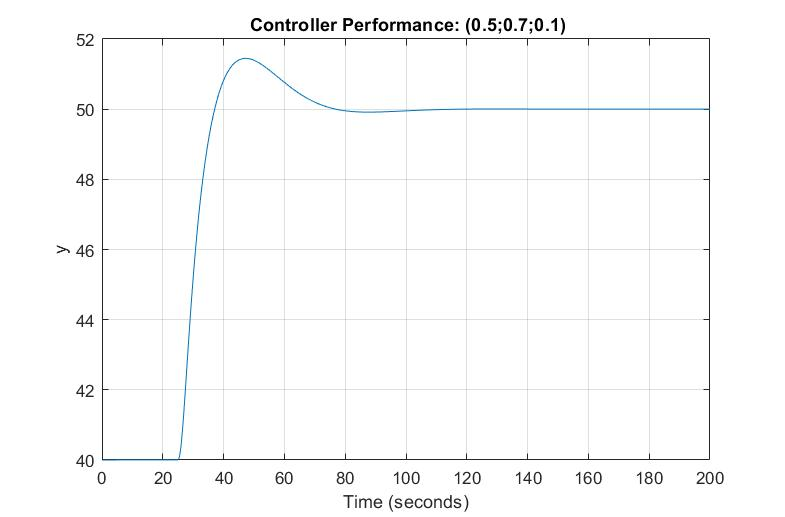
\includegraphics[width = \textwidth]{ex_5_1m}
\caption{Controller Performance for Case 1}
\end{subfigure}
\vspace{1em}
\begin{subfigure}{0.4\textwidth}
  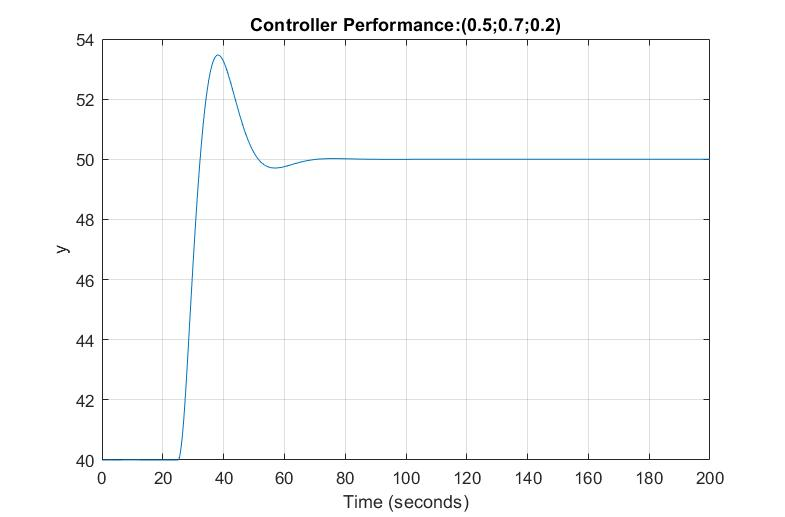
\includegraphics[width = \textwidth]{ex_5_2m}
\caption{Controller Performance for Case 2}
\end{subfigure}
\vspace{1em}
\begin{subfigure}{0.4\textwidth}
 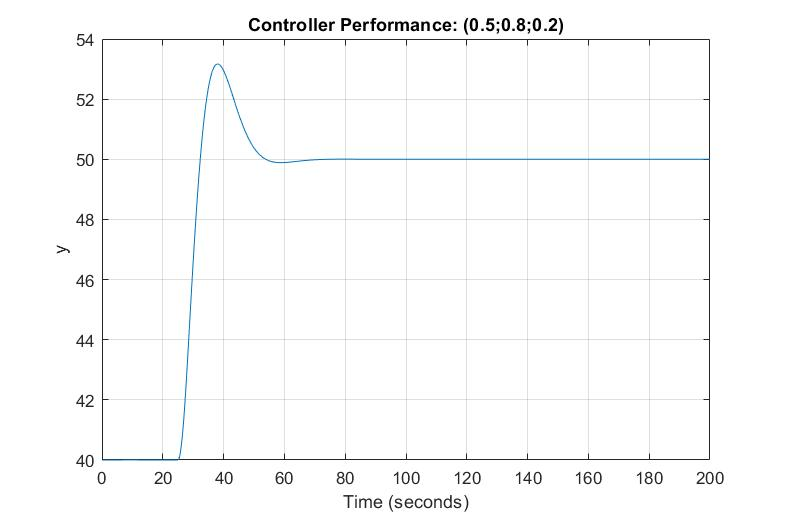
\includegraphics[width = \textwidth]{ex_5_3m}
\caption{Controller Performance for Case 3}
\end{subfigure}
\caption{\textbf{Simulation Results}}
\end{figure} 

The system has some step response characteristics requirements on the closed loop system such as $T\textsubscript{r} < 6s ; M < 35\% ;  T\textsubscript{set} < 30s$ \\
Thus, from the above table it is evident that the 3\textsuperscript{rd} parameter setting of $\chi = 0.5; \zeta = 0.8; \omega \textsubscript{0} = 0.2$ gives the best control performance as a control system with less overshoot, small rise-time and small settling-time is desirable.


\section*{Task 6}

The gain cross over frequency of the open loop system (for the third controller configuration) is 0.362 rad/sec with Phase Margin of 55.3\degree(see fig. \ref{fig:Bode} ).
In order to calculate it, we need to analyze the Bode Plot. The frequency at which the open loop gain first reaches 1 is the gain cross over frequency$( \omega \textsubscript{gc})$ i.e it is the frequency at which the Phase Margin is calculated. 

\begin{figure}[H]
\centering
  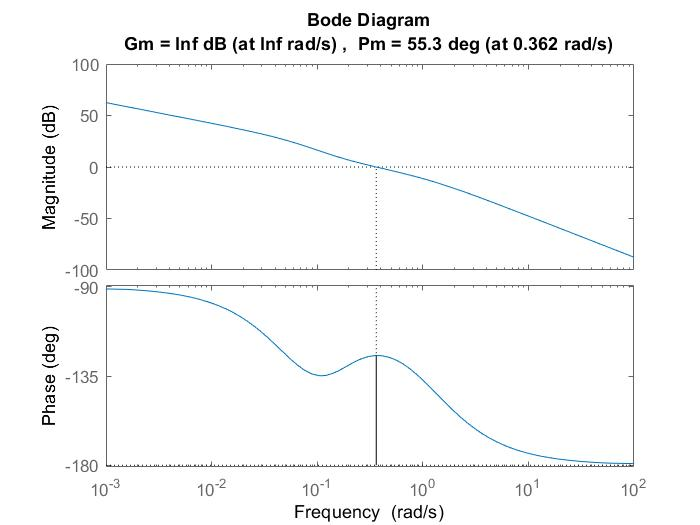
\includegraphics[width = 0.5\textwidth]{ex_6}
\caption{\textbf{Bode Plot of Open Loop System}}
\label{fig:Bode}
 \end{figure}



\section*{Task 7}

\begin{figure}[H]
\centering
\begin{subfigure}{0.4\textwidth}
  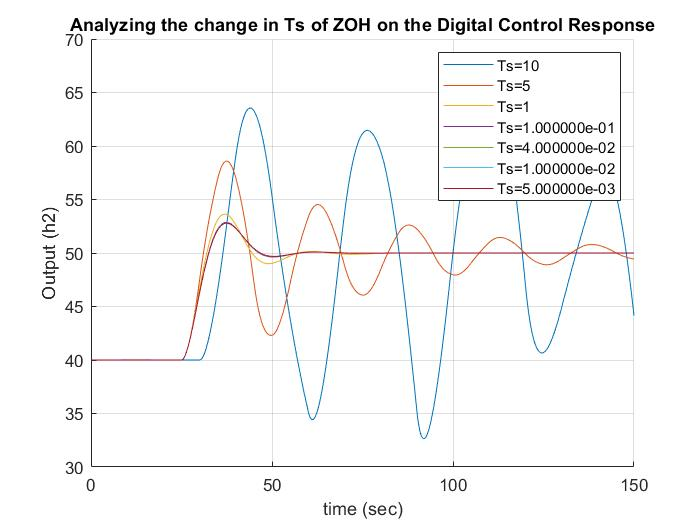
\includegraphics[width = \textwidth]{ex_7_2}
\caption{System Response with ZOH (Various Ts)}
\end{subfigure}
\vspace{1em}
\begin{subfigure}{0.4\textwidth}
  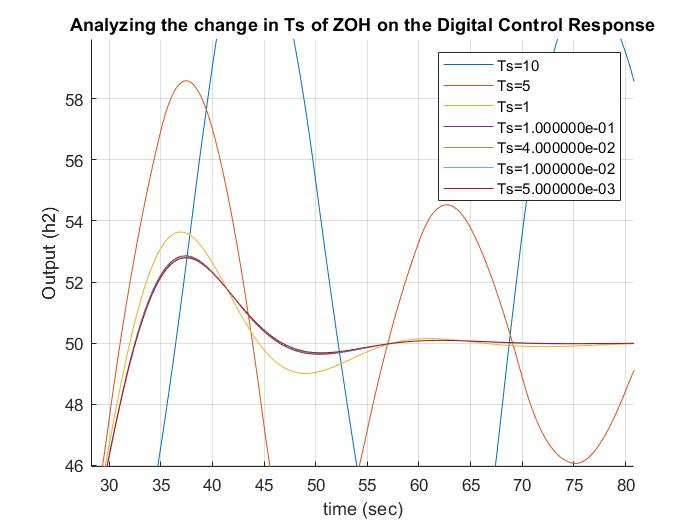
\includegraphics[width = \textwidth]{ex_7_4}
\caption{Peaks of the System Response with ZOH}
\end{subfigure}
\vspace{1em}
\begin{subfigure}{0.4\textwidth}
 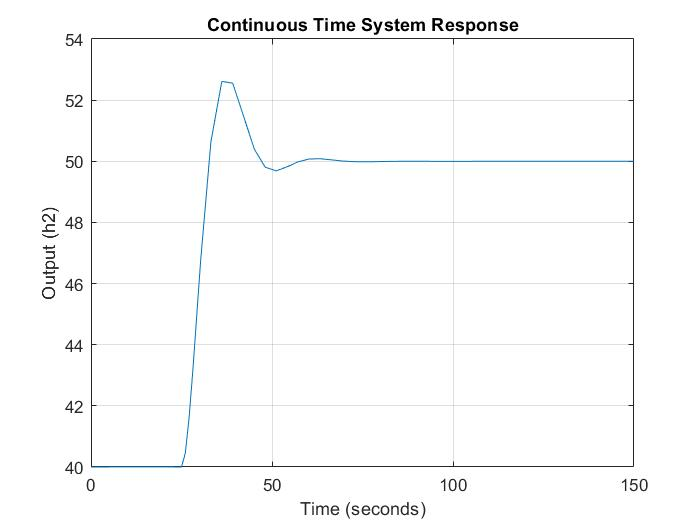
\includegraphics[width = \textwidth]{system_response}
\caption{Continuous Time System Response}
\end{subfigure}
\caption{\textbf{Differences in Control Performance}}
\end{figure}  

From figure (2), we can see that the system time responses for various sampling times : $T \textsubscript{s} = \{10, 5, 1, 0.1, 0.04, 0.01, 0.005\}$ are plotted. 
It has been observed that for very high sampling time of the ZOH, the time response is very oscillatory with a lot of overshoot . As we further reduce the sampling time, the damping increases leading to reduction in the peak overshoot and the settling time. Around a T \textsubscript{s} of 0.005 sec or less, the system starts behaving similar to the continuous time close-loop system but with some more overshoot and delayed settling time mainly due to the delay introduced by the Zero-order Hold.

\section*{Task 8}

\begin{figure}[H]
\centering
\begin{subfigure}{0.4\textwidth}
  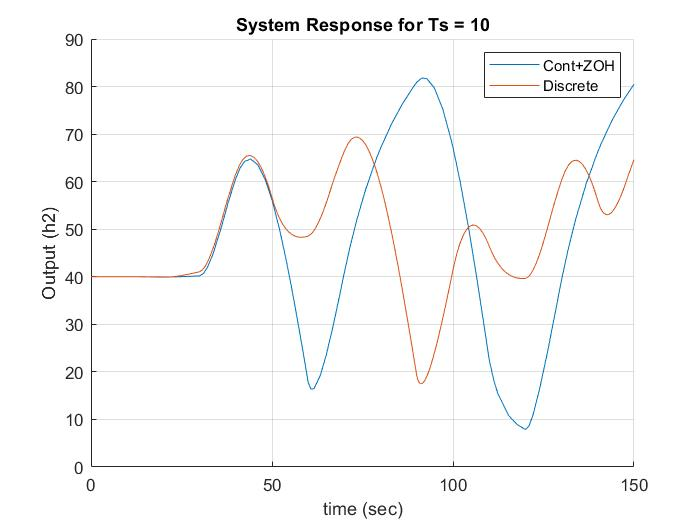
\includegraphics[width = \textwidth]{ex_8_1}
\caption{System Response for T\textsubscript{s} = 10 sec}
\end{subfigure}
\vspace{1em}
\begin{subfigure}{0.4\textwidth}
  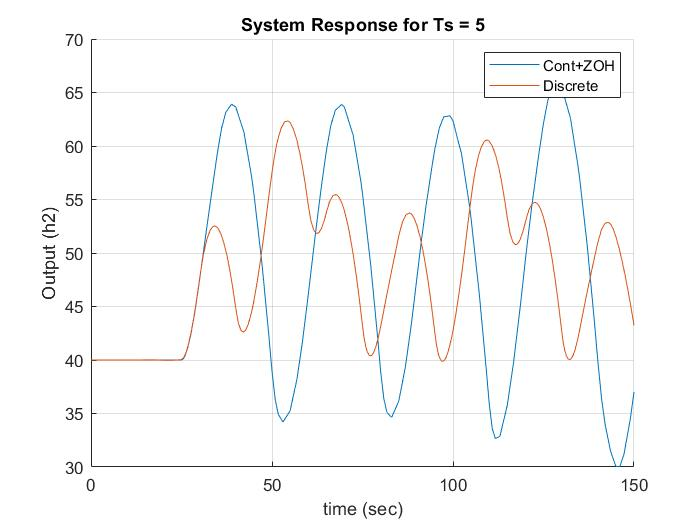
\includegraphics[width = \textwidth]{ex_8_2}
\caption{System Response for T\textsubscript{s} = 5 sec}
\end{subfigure}
\vspace{1 em}
\begin{subfigure}{0.4\textwidth}
  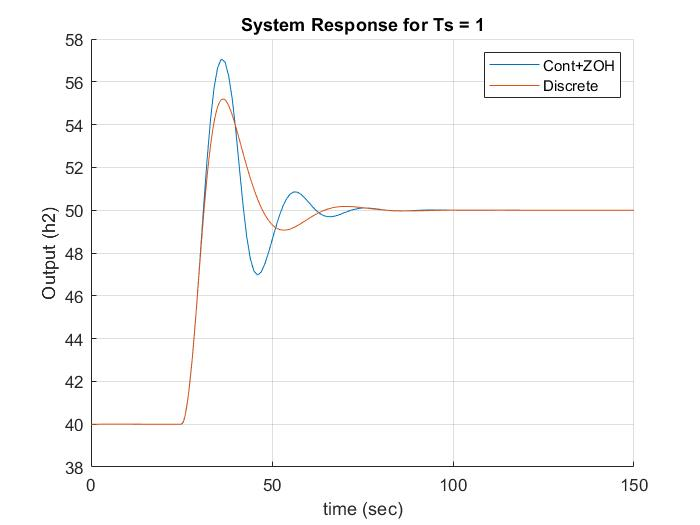
\includegraphics[width = \textwidth]{ex_8_3}
\caption{System Response for T\textsubscript{s} = 1 sec}
\end{subfigure}
\vspace{1em}
\begin{subfigure}{0.4\textwidth}
  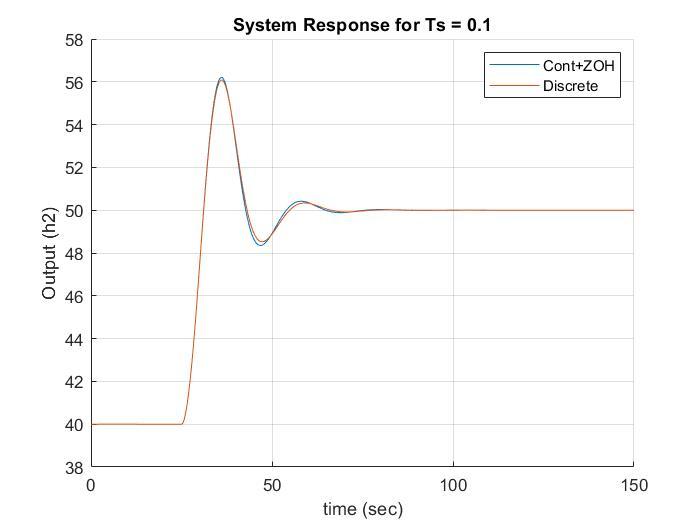
\includegraphics[width = \textwidth]{ex_8_4}
\caption{System Response for T\textsubscript{s} = 0.1 sec}
\end{subfigure}
\vspace{1em}
\begin{subfigure}{0.4\textwidth}
  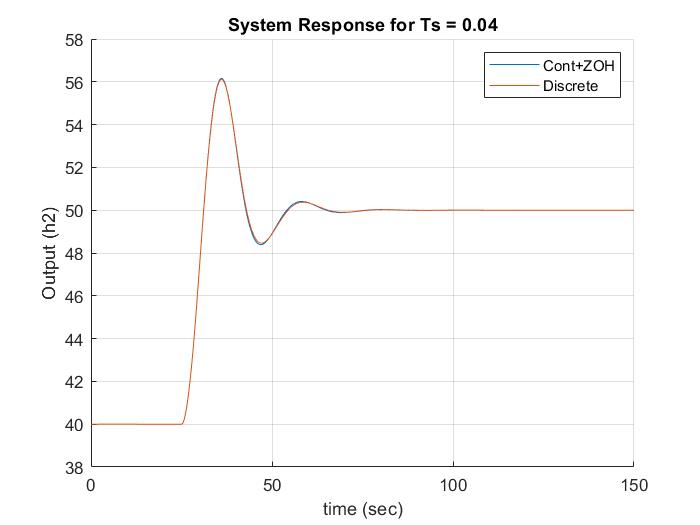
\includegraphics[width = \textwidth]{ex_8_5}
\caption{System Response for T\textsubscript{s} = 0.04 sec}
\end{subfigure}
\vspace{1em}
\begin{subfigure}{0.4\textwidth}
  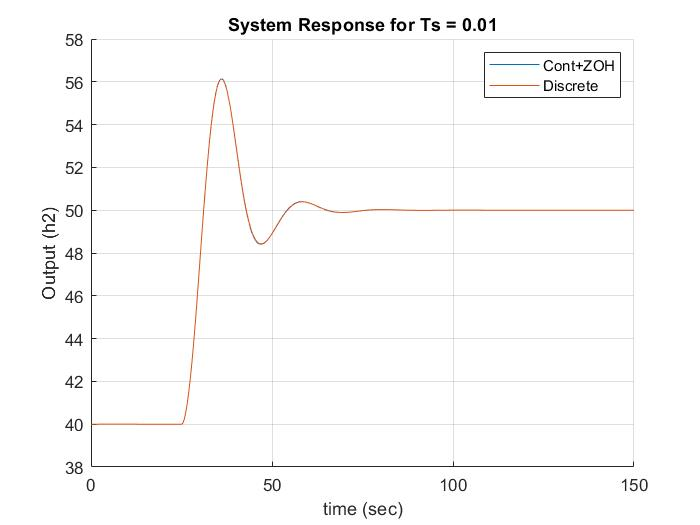
\includegraphics[width = \textwidth]{ex_8_6}
\caption{System Response for T\textsubscript{s} = 0.01 sec}
\end{subfigure}
\vspace{1em}
\begin{subfigure}{0.4\textwidth}
  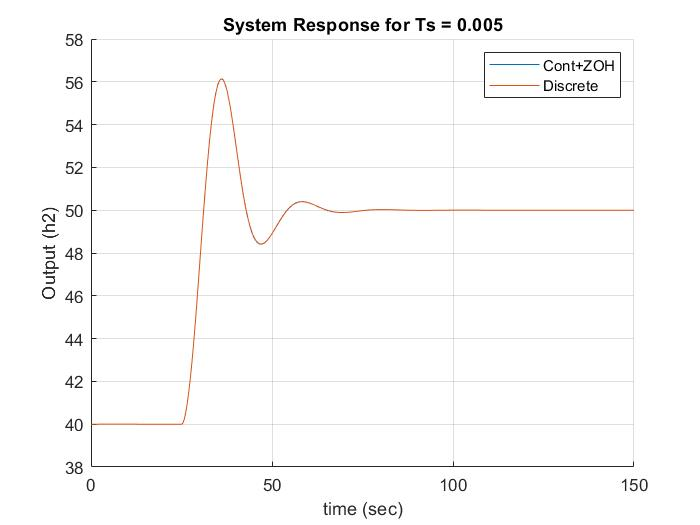
\includegraphics[width = \textwidth]{ex_8_7}
\caption{System Response for T\textsubscript{s} = 0.005 sec}
\end{subfigure}
\caption{\textbf{Differences in Control Performance}}
\label{fig:task8}
\end{figure}  

From the simulation results (\textit{see fig.( \ref{fig:task8})}), we can see that as the Sampling time (T\textsubscript{s}) is decreased, the system stability increases which is evident from the sub-figures (a), (b), (c), and (d). For T\textsubscript{s} = 1 sec, we can see that though the peak overshoot of the discretized controller is lesser than the continuous + ZOH, the response is sluggish. As the T\textsubscript{s} is further reduced the Settling Time (T\textsubscript{set}) of discretized controller reduces and the overall system response comes closer and closer to match that of the Continuous Controller + ZOH. Around T\textsubscript{s} = 0.04 or lower, we can observe that the response of both the controller overlap each other.

\section*{Task 9}

When implementing a continuous controller digitally, we should choose the T\textsubscript{s} such that
 \begin{align*}
 T\textsubscript{s}*\omega \textsubscript{c} \approx 0.05 \  to  \  0.14 
 \end{align*}
\begin{center}
In the Task 6, we calculated $\omega \textsubscript{c} = 0.362 \ rad/sec $ \\ 
Thus, $T\textsubscript{s} \ lies \ in \ the \ range \ of \approx 0.138 \ and \ 0.3867$
\end{center}

\section*{Task 10}

\begin{center}
\textit{Considering the controller parameters with $\chi = 0.5; \ \omega \textsubscript{0} = 0.2; \ \zeta =0.8$ } \\
\end{center}
The maximum possible sampling time without affecting the control performance of a system with discretized controller is observed to be around 0.4 sec. But from  T\textsubscript{s} = 0.5 sec to 1.5 sec, the performance of the system deteriorated a little in terms of sluggish nature i.e low T\textsubscript{r} and T\textsubscript{set} but as I increased the T\textsubscript{s} above this, it deteriorated exponentially till the point of becoming very oscillatory around T\textsubscript{s} = 5 sec and diverging above T\textsubscript{s} = 10 sec.
The theoretically calculated maximum T\textsubscript{s} was 0.3867 which is very near to what is observed from the simulation results. But depending upon how much compromise in the performance is fine, this upper limit can be extended a little.

\section*{Task 11}

\begin{figure}[H]
\centering
  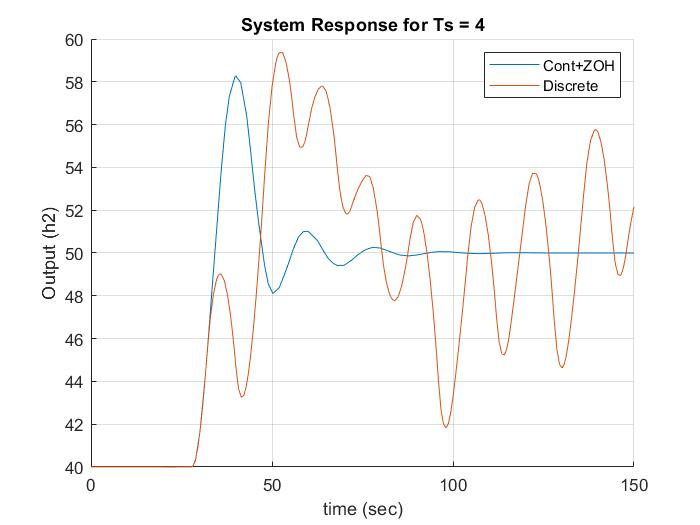
\includegraphics[width = 0.5\textwidth]{ex_11_new}
\caption{\textbf{Control Performance for T\textsubscript{s} = 4 sec}}
 \end{figure}

For the mentioned sampling time of 4 sec, the control performance of the discretized controller system is highly oscillatory. On the other hand, if we consider the case with Continuous + ZOH controller, it settles down after some initial oscillations.

\section*{Task 12}

The Linearized System Equation was first converted from Laplace Domain to Time Domain and then expressed in state-space form to obtain :
\[
A = 
\begin{bmatrix}
  -1/Tau & 0 \\
  1/Tau & -1/(gamma \_ tank*Tau)
\end{bmatrix}
\]
\[
B = 
\begin{bmatrix}
  k \_ tank/Tau  \\
0
\end{bmatrix}
\]
\[
C = 
\begin{bmatrix}
  0 & 1
\end{bmatrix}
\]
\[
D = 
\begin{bmatrix}
  0
\end{bmatrix}
\]

The State-Space form of the Continuous system was discretized with T \textsubscript{s} = 4 sec and the Discrete-time State Space matrices were derived as follows:
\[
\Phi = 
\begin{bmatrix}
  0.7249 & 0 \\
  0.2332 & 0.7249
\end{bmatrix}
\]
\[
\Gamma = 
\begin{bmatrix}
  0.6017  \\
  0.0916
\end{bmatrix}
\]
\[
C = 
\begin{bmatrix}
  0 & 1
\end{bmatrix}
\]
\[
D = 
\begin{bmatrix}
  0
\end{bmatrix}
\]

\section*{Task 13}

The observability and reachability of the discrete-time plant model was checked using MATLAB. 
\begin{lstlisting}
% Observability and reachability
Wo = obsv(Phi,C)
isObsv = length(Phi) - rank(Wo)
Wc = ctrb(Phi,Gamma)
isCtrb = length(Phi) - rank(Wc)
\end{lstlisting}

After executing the above code snippet, we got
\[
W\textsubscript{o} = 
\begin{bmatrix}
  0 & 0.0142 \\
  0.0142 & 0.0136
\end{bmatrix}
\]
\[
W\textsubscript{c} =
\begin{bmatrix}
  2.8993 & 1.3037 \\
 6.4741 & 14.6090
\end{bmatrix}
\]
Also,
\begin{align*}
isObsv = 0 \\
isCtrb = 0
 \end{align*}
which means that the Observability matrix and Reachability matrix has full rank and the discrete-time plant is \textbf {Observable} and \textbf {Reachable}.
\section*{Task 14}

The reference gain \textit l\textsubscript{r} is necessary in order to ensure that the steady state output $y \textsubscript {e} = r$ i.e it ensures that we are able to design the dynamics of the system to satisfy our goal.

\section*{Task 15}

The state-space equation for the dynamic observer is as follows:
\begin{align}
\Delta \hat{x}(k+1) &= \Phi \ \Delta  \hat{x}(k) + \Gamma \ \Delta u(k) + K \ [\Delta y \ - \  C \ \Delta \hat{x}(k)] \\
\Delta y \ &= C \ \Delta x(k) \\ 
\therefore \  \Delta \hat{x}(k+1) &= [\Phi \ - \ KC] \ \Delta  \hat{x}(k) + \Gamma \ \Delta u(k) + K C \ \Delta x(k) \\
\end{align}
Now plugging in the Control Law of the form
\begin{equation}
\Delta u(k) = -L \ \Delta  \hat{x}(k) + l \textsubscript{r} \ r(k) \\ 
\end{equation}
We get, \\
\begin{equation}
\Delta \hat{x}(k+1) = [\Phi \ - \ KC \ -\Gamma L] \ \Delta  \hat{x}(k) + \Gamma \ l \textsubscript{r} \ r(k) + K C \ \Delta x(k) \\
\end{equation}

The state-space form of the original system is given by
\begin{equation}
\Delta x(k+1) = \Phi \ \Delta  x(k) + \Gamma \ \Delta u(k) 
\end {equation}

Now, plugging in the Control Law $\Delta u(k)$, we get
\begin{equation}
\Delta x(k+1) = \Phi \ \Delta  x(k) \ - \ \Gamma L \ \Delta \hat{x}(k)  \ + \ \Gamma \ l\textsubscript{r} \  r(k)
\end {equation}

Thus, representing the eq.(5) and eq.(10) in a state-space form, we get
\[
\begin{bmatrix}
  \Delta x(k+1) \\
 \Delta \hat{x}(k+1)
\end{bmatrix}
=
\begin{bmatrix}
 \Phi & -\Gamma L \\
K C & \Phi-K C-\Gamma L
\end{bmatrix}
\begin{bmatrix}
  \Delta x(k) \\
 \Delta \hat{x}(k)
\end{bmatrix}
+
\begin{bmatrix}
\Gamma l\textsubscript{r} \\
\Gamma l\textsubscript{r} 
\end{bmatrix}
r(k)
\]

Comparing this equation with $x\textsubscript{a}(k+1) = A\textsubscript{a} \ x\textsubscript{a}(k) + B\textsubscript{a} \ r(k)$

We get,

\[
A\textsubscript{a} = 
\begin{bmatrix}
\Phi & -\Gamma L \\
K C & \Phi-K C-\Gamma L
\end{bmatrix}
\]
\[
B\textsubscript{a} = 
\begin{bmatrix}
  \Gamma l\textsubscript{r} \\
\Gamma l\textsubscript{r} 
\end{bmatrix}
\]

\section*{Task 16}

Let $\Delta \tilde{x}(k) = \Delta x(k) - \Delta \hat{x}(k)$
 Thus, substituting for $\Delta \hat{x}(k)$ in eq.(10), we get 
\begin{equation}
\Delta x(k+1) = [\Phi \  - \ \Gamma L] \ \Delta  x(k)  \ + \  \Gamma L \ \Delta \tilde{x}(k) \ + \ \Gamma \ l\textsubscript{r} \  r(k) \\
\end{equation}

Now, from eq.(3), eq.(4)and eq.(7), we get
\begin{equation}
\Delta \hat{x}(k+1) = \Phi \ \Delta  \hat{x}(k) \ - \ \Gamma L \ \Delta \hat{x}(k) \ + \ \Gamma \ l\textsubscript{r} r(k) \ + \ K C \ \Delta \tilde{x}(k) \\
\end{equation}

Substituting for $\Delta \hat{x}(k)$ in eq.(12), we get 
\begin{equation}
\Delta \tilde{x}(k+1) = [\Phi \ - K C] \ \Delta \tilde{x}(k)
\end{equation}

Expressing the above equations in state-space form, we get
\[
\begin{bmatrix}
  \Delta x(k+1) \\
 \Delta \tilde{x}(k+1)
\end{bmatrix}
=
\begin{bmatrix}
  \Phi - \Gamma L &  \Gamma L \\
  0 & \Phi - KC
\end{bmatrix}
\begin{bmatrix}
  \Delta x(k) \\
 \Delta \tilde{x}(k)
\end{bmatrix}
+
\begin{bmatrix}
\Gamma l\textsubscript{r} \\
0
\end{bmatrix}
r(k)
\]

Let 
\[
z(k) = 
\begin{bmatrix}
  \Delta x(k) \\
 \Delta \tilde{x}(k)
\end{bmatrix}
\]

Thus, the above state-space representation can be re-written as:

\[
z(k+1) = 
\begin{bmatrix}
  \Phi - \Gamma L &  \Gamma L \\
  0 & \Phi - KC
\end{bmatrix}
z(k) +
\begin{bmatrix}
 \Gamma \textit l\textsubscript{r}\\
  0
\end{bmatrix}
r(k)
\]

Now if we try to find the eigen values of the above system, we get 
\begin{equation}
[sI - (\Phi - \Gamma L)] [sI - (\Phi - KC)] = 0 \\
\end{equation}

Thus pole placement for both can be done independently, which shows that Separation Principle holds.

\section*{Task 17}
The Simulink model with the Continuous Controller was linearized using the Linear Model Analysis Toolkit and that model was exported to the MATLAB workspace. For this task, we used the 3\textsuperscript{rd} controller specification with $\chi = 0.5; \ \omega \textsubscript{0} = 0.2; \ \zeta =0.8$. 
The eigen values of the Linearized Continuous time closed loop system were as follows: \\
$p = [-0.5176, -0.4822, -0.1601+0.1201i, -0.1601-0.1201i ]$ 

These poles were converted into discrete-time using the equation 
\begin{align*}
z\textsubscript{i} &= e^{T\textsubscript{s} \ p\textsubscript{i}} ... \forall T\textsubscript{s} = 4 sec.\\
\implies z\textsubscript{i} &= [0.1261, 0.1453, 0.4675+0.2436i, 0.4675-0.2436i]
\end{align*}

Owing to the Separation Principle, the Controller as well as the Observer can be designed independently. Coming to the observer, as the control action depends upon the state estimation by observer, it has to be faster than the controller. Also, theoretically the observer error will decrease if the poles of s-plane are further to the left. On the other hand for the State feedback Controller, the dominant poles in the s-plane are used as they have more impact on the system transient response. 
The Controller gain \textbf{L} and Estimator gain \textbf K values were calculated using the \verb acker \  function.  We have also verified that the A\textsubscript{a} has the desired poles(z-domain) [0.1261, 0.1453, 0.4675+0.2436i, 0.4675-0.2436i].

\begin{lstlisting}
% MATLAB code for Task 17

p_controller = [0.4675+0.2436i 0.4675-0.2436i];
p_observer = [0.1261 0.1453];
L = acker(Phi,Gamma,p_controller);
M = acker(Phi',C',p_observer);

% reference gain
num = 1;
den1 = C/(eye(2)-Phi+(Gamma*L));
den = den1 * Gamma;
lr = num / den;

% augmented system matrices
Aa = [Phi -(Gamma*L); M'*C Phi-(Gamma*L)-(M'*C)];
Ba = [Gamma.*lr; Gamma.*lr];
\end{lstlisting}

\section*{Task 18}

\begin{figure}[H]
\centering
  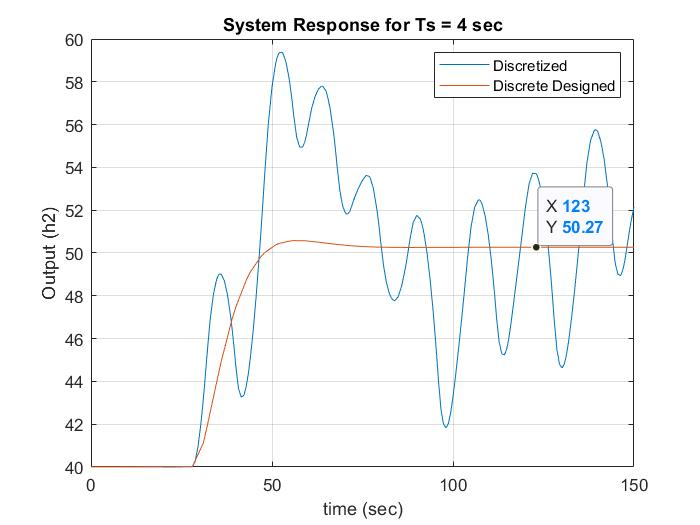
\includegraphics[width = 0.5\textwidth]{ex_18_new}
\caption{\textbf{Control Performance for T\textsubscript = 4 sec}}
 \end{figure}
From Figure (5), we can see that the performance of the system has improved a lot (oscillations have reduced to a great extent and T\textsubscript{s} has also reduced) for the discrete designed controller system. This may be because this controller is specifically designed for the discrete system and has been designed to place the closed loop discrete poles at the desired location by considering State Feedback as well as Estimator design. \\
The time-response of the discrete designed system settles down having a steady-state error value of \textbf {0.27}.  There is a small steady-state error in the output which maybe because of the following reasons
\begin{itemize}
\item The type number of the system is zero and hence, for a step input the steady-state error is non-zero.
\item As the Observer Gain takes large values, there is a possibility of noise amplification.
\end{itemize}

\section*{Task 19}

Quantization with 10 bits is  abs(\(\frac{0-100}{2^{10}}\)) = 0.0976.

\section*{Task 20}

A Quantization block was successfully constructed in Simulink by connecting a Quantizer block to a Saturation block. The Saturation block is necessary because the only parameter that the Quantizer block has is the Quantization Interval and no upper or lower limit. Thus, in order to limit the signal between the desired limits, we add a Saturation block.

\section*{Task 21}
Different Quantization levels [12.5, 6.25, 1.56, 0.78125, 0.39, 0.097] corresponding to [3, 4, 6, 7, 8, 10] bits were used to simulate the system. 
 \begin{figure}[H]
\centering
  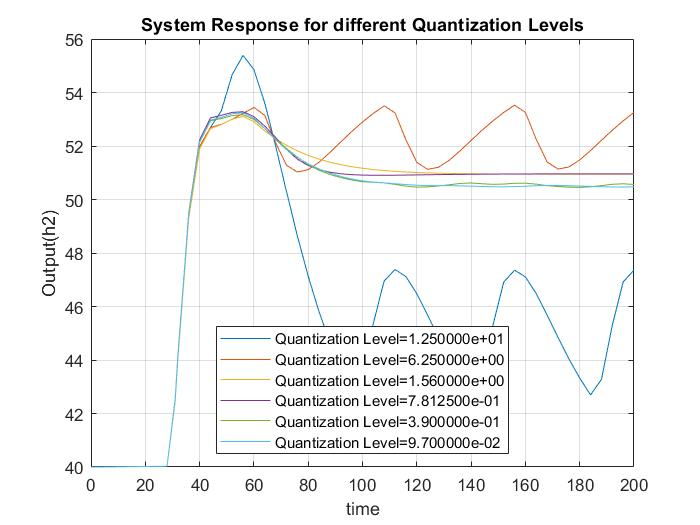
\includegraphics[width = 0.5\textwidth]{ex_21}
\caption{\textbf{System Response for different Quantization Levels }}
 \end{figure}

From figure (6), we can observe that for Quantization levels greater than \textbf{0.78125} (corresponding to lower than 7 bits), the control performance starts to degrade.
The Simulink model with Quantization Subsystem consisting of Quantizer in series with Saturation is shown below:
\begin{figure}[H]
\centering
  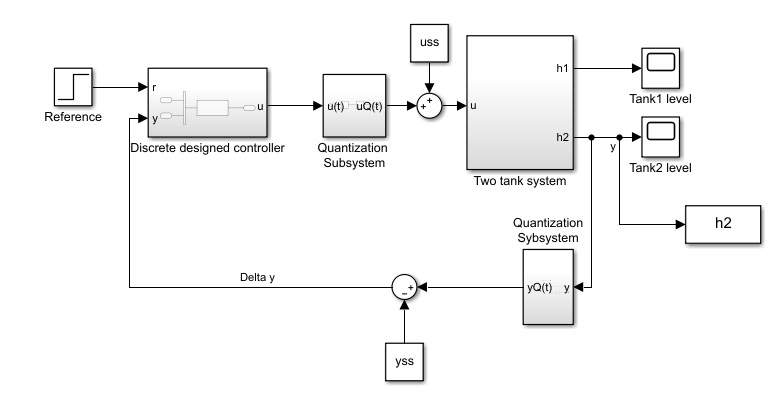
\includegraphics[width = 0.5\textwidth]{simModel}
\caption{\textbf{Simulink Tank Model with Quantization blocks }}
 \end{figure}

\end{document}      % End of the document
